\documentclass[12pt]{article}
\usepackage{graphicx}
\usepackage[euler-digits]{eulervm}
\usepackage{charter,amsmath,amssymb,breakurl}
\usepackage[letterpaper,margin=1in]{geometry}
\title{Math 265 Quiz 1}\author{}\date{}
\begin{document}
\maketitle
\thispagestyle{empty}
\begin{enumerate}
\item Find a unit vector with the same direction as
$8\mathbold{i}-\mathbold{j}+4\mathbold{k}$.
\vspace{1in}
\item Calculate $\mathsf{proj}_\mathbold{w}\mathbold{v}$
where $\mathbold{v}=\left\langle 3,4,0\right\rangle$ and
$\mathbold{w}$ is the vector from $\left(1,1,0\right)$
to $\left(11,12,-2\right)$.
\vspace{2in}
\item
A water main is to be constructed with a $20^\circ$~grade in the north
direction and a $10^\circ$~grade in the east direction, as shown in the
figure below. Calculate the angle between the two pipes
at the point where the main changes from north to east.
\vspace{1in}

\hfill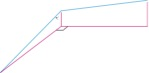
\includegraphics{Water}

\end{enumerate}
\end{document}
